% ScienceMontgomery poster - 48" x 36" landscape (beamerposter)
% Upload this folder to Overleaf and compile with PDFLaTeX.
% Requires the beamerposter package (bundled with most TeX distributions / Overleaf).
\documentclass[final]{beamer}
\mode<presentation>
\usepackage[orientation=landscape,size=custom,width=121.92,height=91.44,scale=1.11]{beamerposter}
\usepackage[T1]{fontenc}

% -- Theme colors (modern-light: navy / coral / gold) --
\definecolor{navy}{RGB}{27,42,74}
\definecolor{paperbg}{RGB}{248,249,250}
\definecolor{surface}{RGB}{255,255,255}
\definecolor{bodytext}{RGB}{34,34,34}

\setbeamercolor{background canvas}{bg=paperbg}
\setbeamercolor{block title}{bg=navy,fg=white}
\setbeamercolor{block body}{bg=surface,fg=bodytext}
\setbeamertemplate{block title}{%
  \vskip2pt\centering\usebeamerfont{block title}\insertblocktitle\vskip2pt}
\setbeamertemplate{navigation symbols}{}
\setbeamerfont{block title}{size=\large,series=\bfseries}
\setbeamerfont{block body}{size=\normalsize}
\setbeamerfont{itemize/enumerate body}{size=\normalsize}
\usepackage{booktabs}
\usepackage[font=small]{caption}
\usepackage[utf8]{inputenc}

\graphicspath{{figures/}}

\title{Cross-Platform Colon Cancer Proliferation Classification}
\author{\footnotesize Ronisnotasianfr --- ScienceMontgomery 2025}
\date{}

\begin{document}
\begin{frame}[t]

\begin{beamercolorbox}[wd=119.2cm,ht=4.8cm,rounded=true]{title}
  \begin{center}
    {\LARGE \textbf{Cross-Platform Colon Cancer Proliferation Classification}}\\[0.25cm]
    {\small Leakage-Free ML Pipeline | StabilitySelector | Calibration Benchmark | Drug Screen}\\[0.15cm]
    {\small Ronisnotasianfr --- ScienceMontgomery 2025}
  \end{center}
\end{beamercolorbox}
\vspace{0.15cm}

% ---------------------------------- 3 COLUMNS ----------------------------------
\begin{columns}[t]

% --------------------------- Column 1 (narrow) ---------------------------
\begin{column}{0.27\textwidth}
\begin{block}{Problem \& Motivation}
Colon cancer is the 2nd leading cause of cancer death worldwide. Ki-67 IHC --- the clinical standard for proliferation assessment --- is subjective, single-gene, and offers no drug prediction.

\textbf{Can ML predict proliferation from transcriptomics without data leakage?}

We address this with a leakage-free pipeline trained on GEO (Affymetrix, $n=585+232$), validated on TCGA-COAD (RNA-seq, $n=329$) and CPTAC (proteomics, $n=105$), and linked to drug sensitivity via GDSC2 (295 drugs $\times$ 969 cell lines).

\textbf{Key Innovation:} a bootstrap-based StabilitySelector that retains features present in top-K across $\geq 50\%$ of 100 resamples, combined with nested cross-validation and anti-leakage gene filtering.
\end{block}

\vspace*{0.25cm}

\begin{block}{Ki-67 Correlation (Leakage-Free)}
\begin{center}
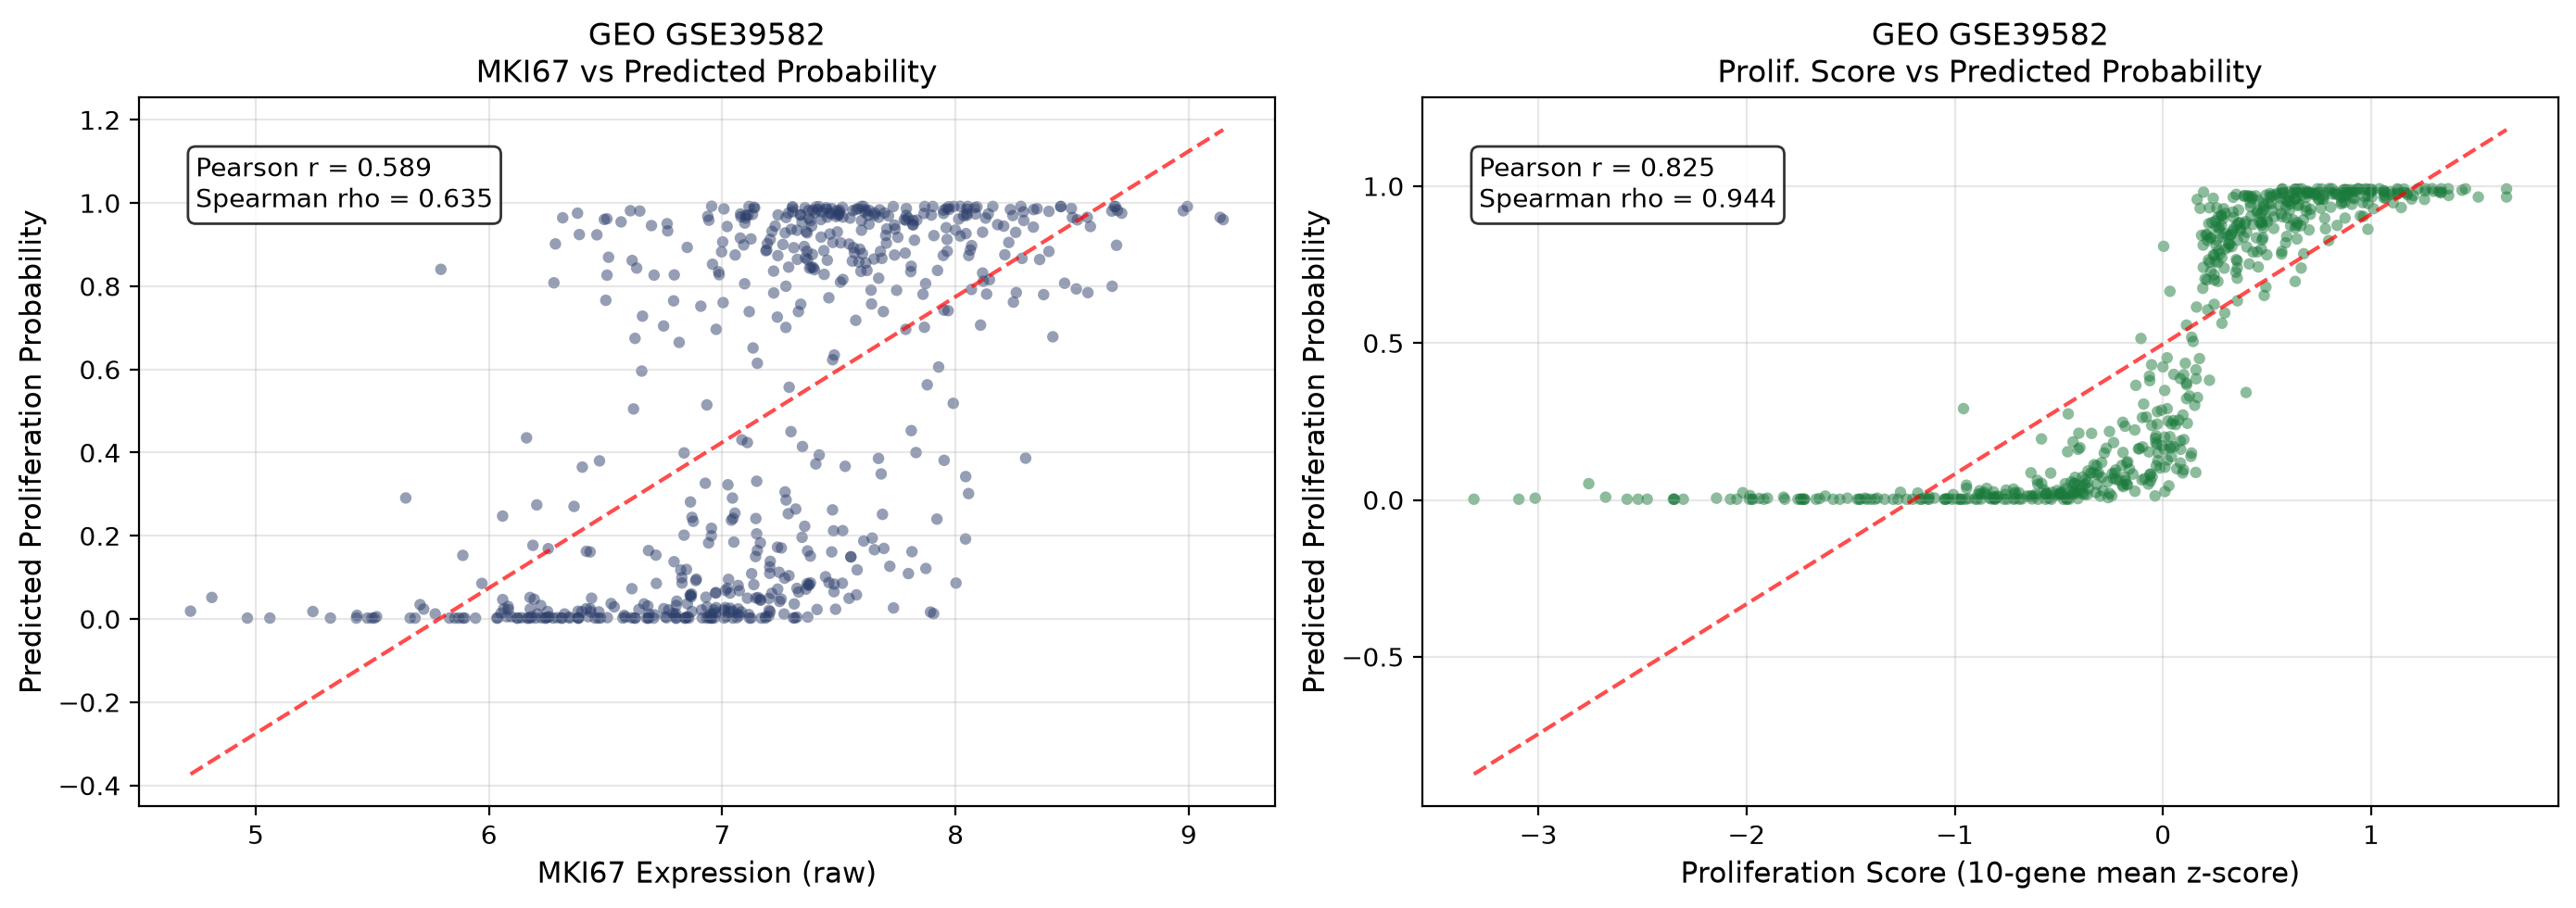
\includegraphics[width=0.60\columnwidth]{ki67_correlation_geo_gse39582.png}
\end{center}
\textbf{GEO:} $r = 0.59$, $p < 10^{-55}$ \quad \textbf{TCGA-COAD:} $r = 0.54$, $p < 10^{-25}$

10 proliferation genes (MKI67, TOP2A, etc.) removed from the feature set. The model infers proliferation via the downstream transcriptional cascade --- not direct Ki-67 proxies.
\end{block}

\vspace*{0.25cm}

\begin{block}{Drug Sensitivity (GDSC2)}
\begin{center}
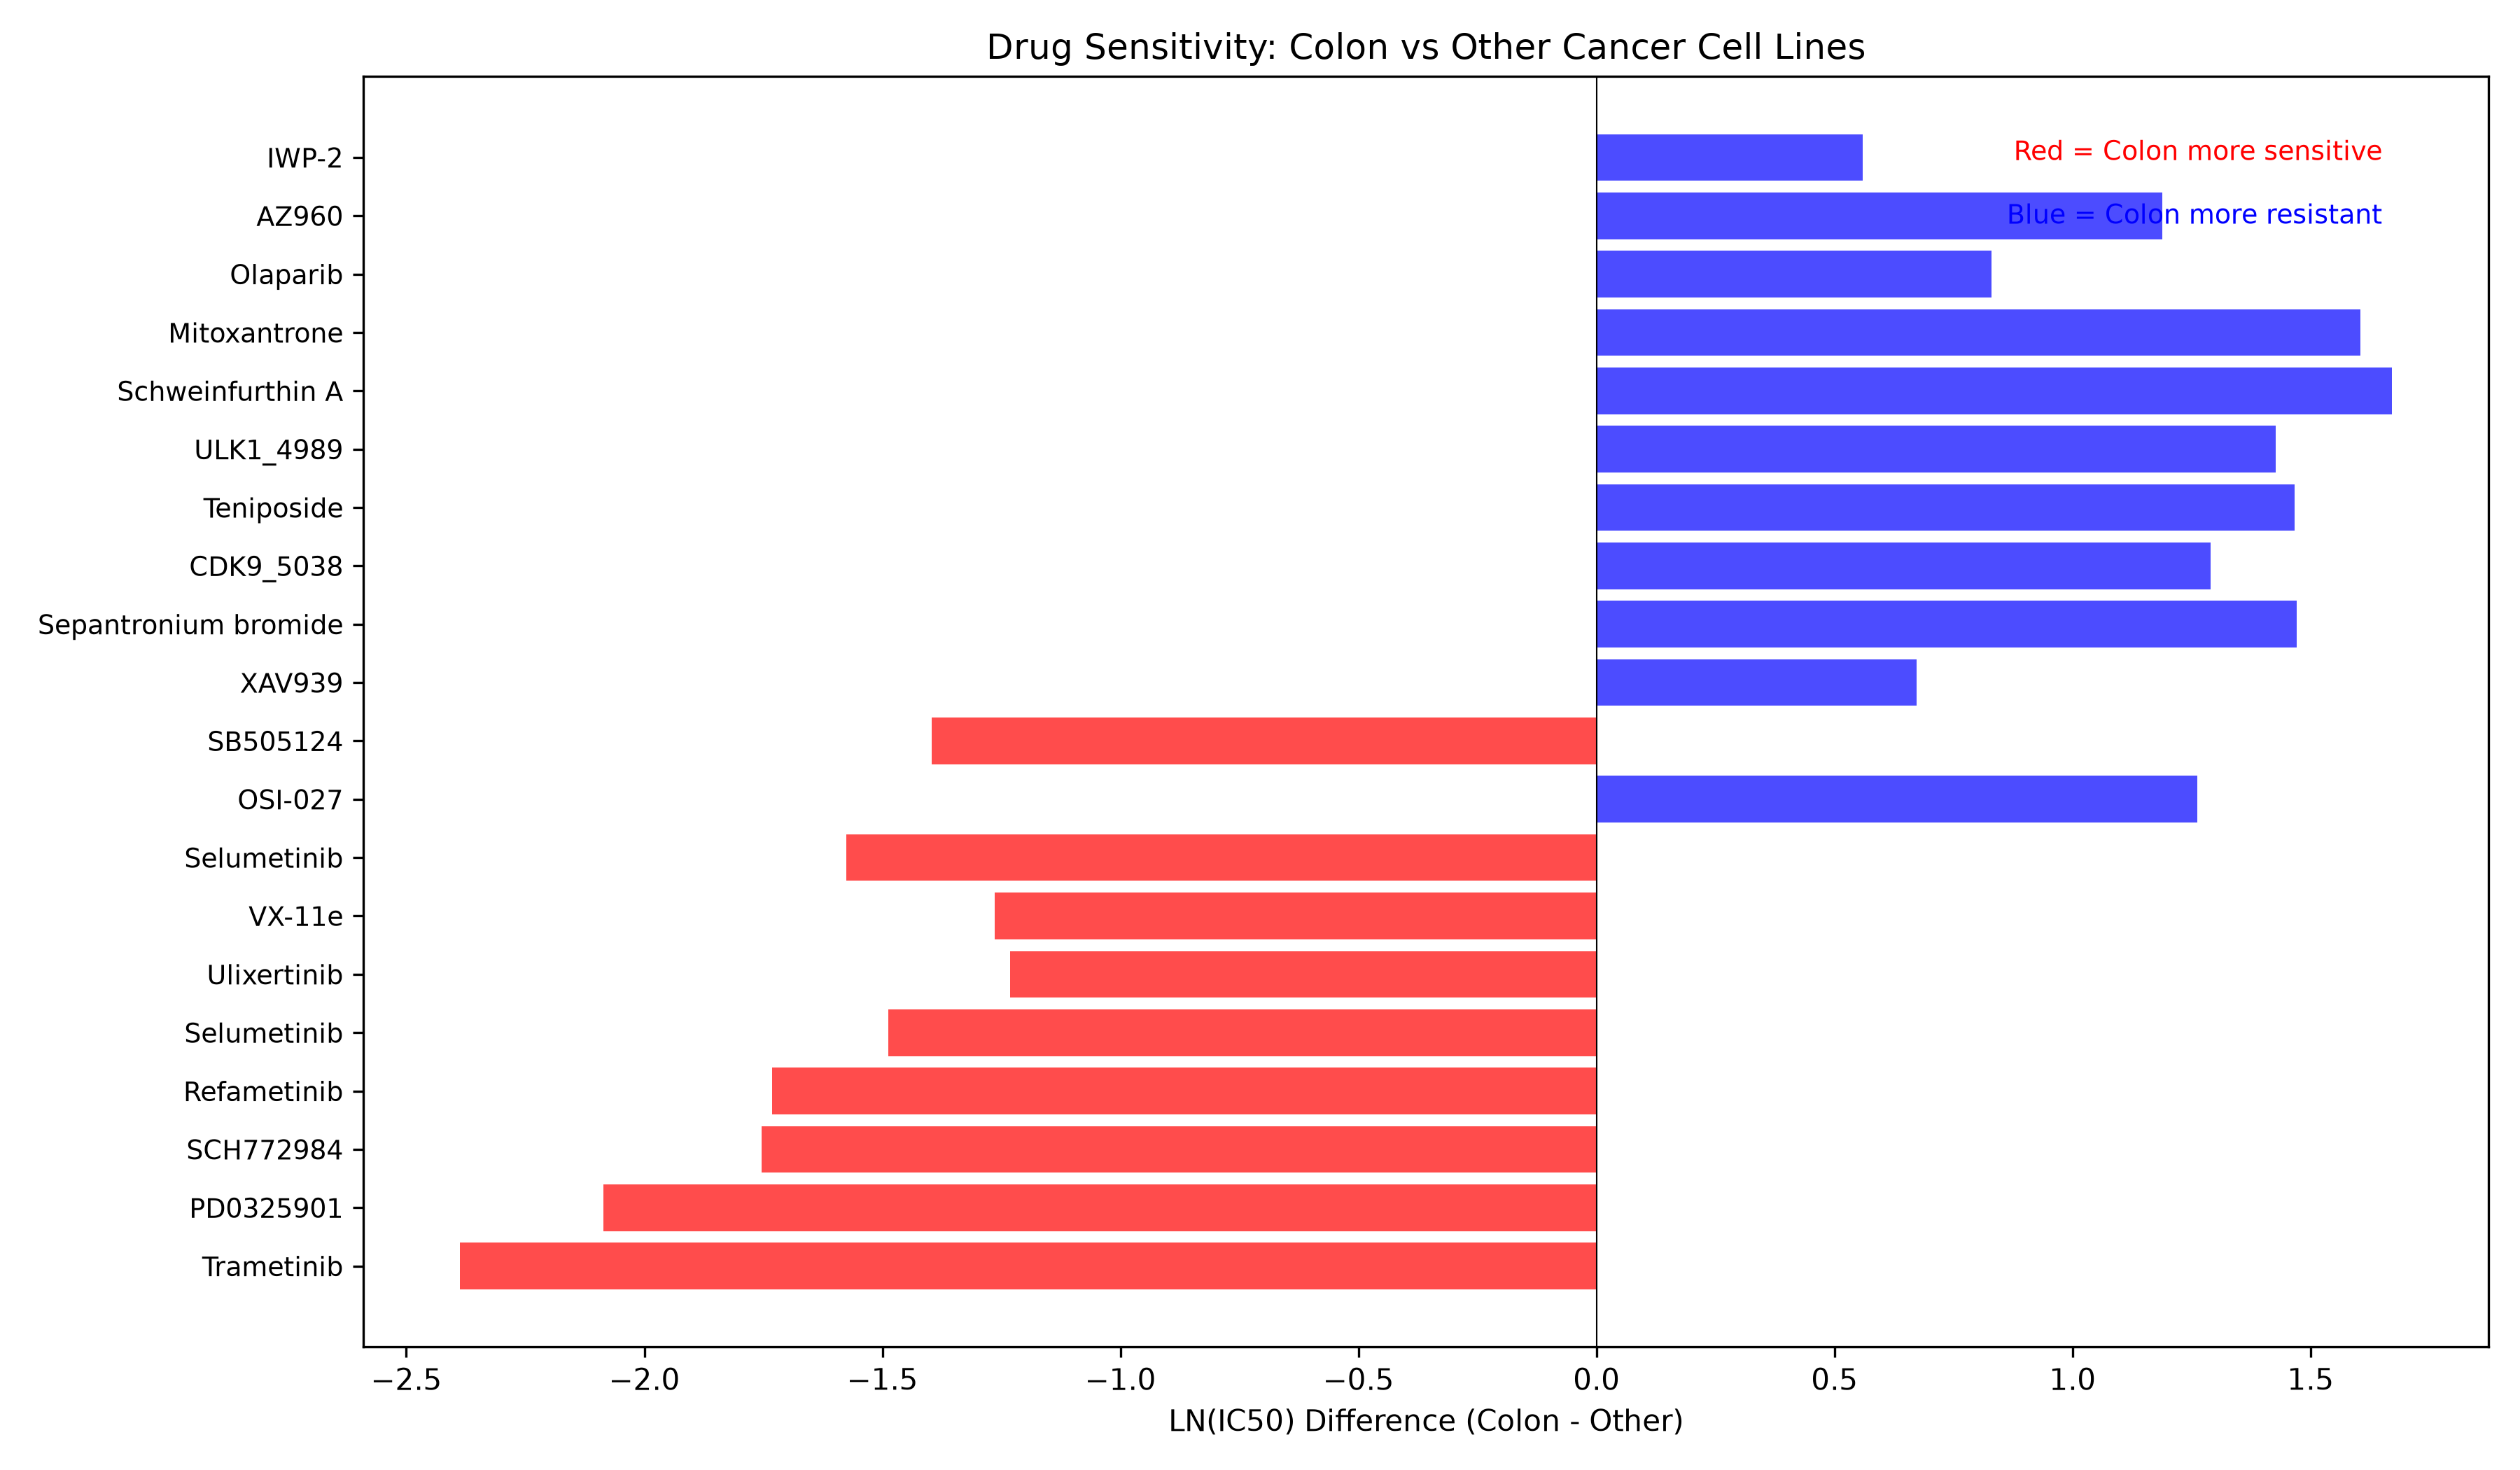
\includegraphics[width=0.73\columnwidth]{drug_sensitivity_top_drugs.png}
\end{center}
\textbf{Bonferroni-corrected: 295 drugs $\times$ 969 cell lines}
\begin{itemize}
\item \textbf{Trametinib (MEK)} --- $p = 1.8\times 10^{-12}$
\item \textbf{PD0325901 (MEK)} --- $p = 5.9\times 10^{-12}$
\item \textbf{SCH772984 (ERK)} --- $p = 1.1\times 10^{-10}$
\item \textbf{Refametinib (MEK)} --- $p = 2.7\times 10^{-10}$
\end{itemize}
\textbf{Top 5 hits all target the MAPK/ERK pathway --- biologically coherent.}
\end{block}

\vspace*{0.25cm}


\begin{block}{Clinical Decision Curve}
\begin{center}
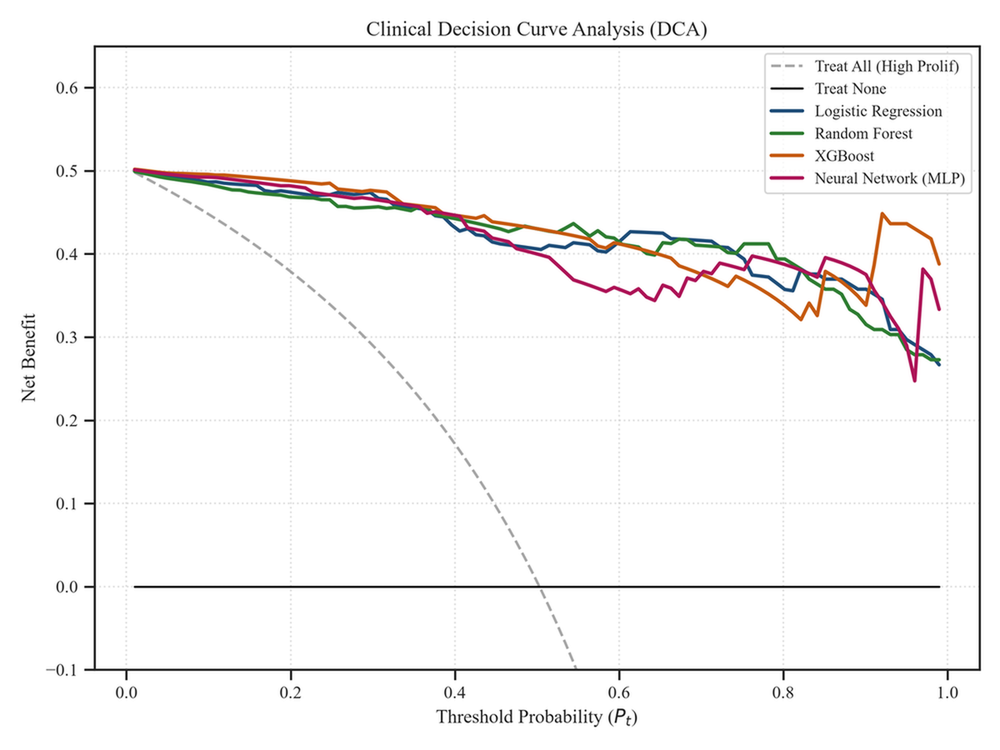
\includegraphics[width=0.88\columnwidth]{clinical_dca.png}
\end{center}
Model-guided management shows \textbf{positive net benefit} across clinically relevant threshold probabilities versus treat-all / treat-none default strategies.
\end{block}
\end{column}

% --------------------------- Column 2 (wide) ---------------------------
\begin{column}{0.38\textwidth}
\begin{block}{Pipeline \& Methodology}
\begin{itemize}
\item \textbf{GEO GSE39582 (585) + GSE17538 (232) $\rightarrow$ train split}
\item \textbf{Remove 10 proliferation genes (anti-leakage guard)}
\item \textbf{StabilitySelector: bootstrap 100$\times$, keep $\geq 50\%$ consensus}
\item \textbf{4 models: LR, RF, XGBoost, MLP with nested CV}
\item \textbf{TCGA-COAD (329) + CPTAC (105) $\rightarrow$ external validation}
\item \textbf{5 calibration methods (Platt, Isotonic, QN, QN+Platt)}
\item \textbf{GDSC2: 295 drugs $\times$ 969 lines (Bonferroni corrected)}
\end{itemize}

\centering Bootstrap 100$\times$ | ANOVA F-scores per resample | Retain features in top-K across $\geq 50\%$ of resamples

\begin{center}
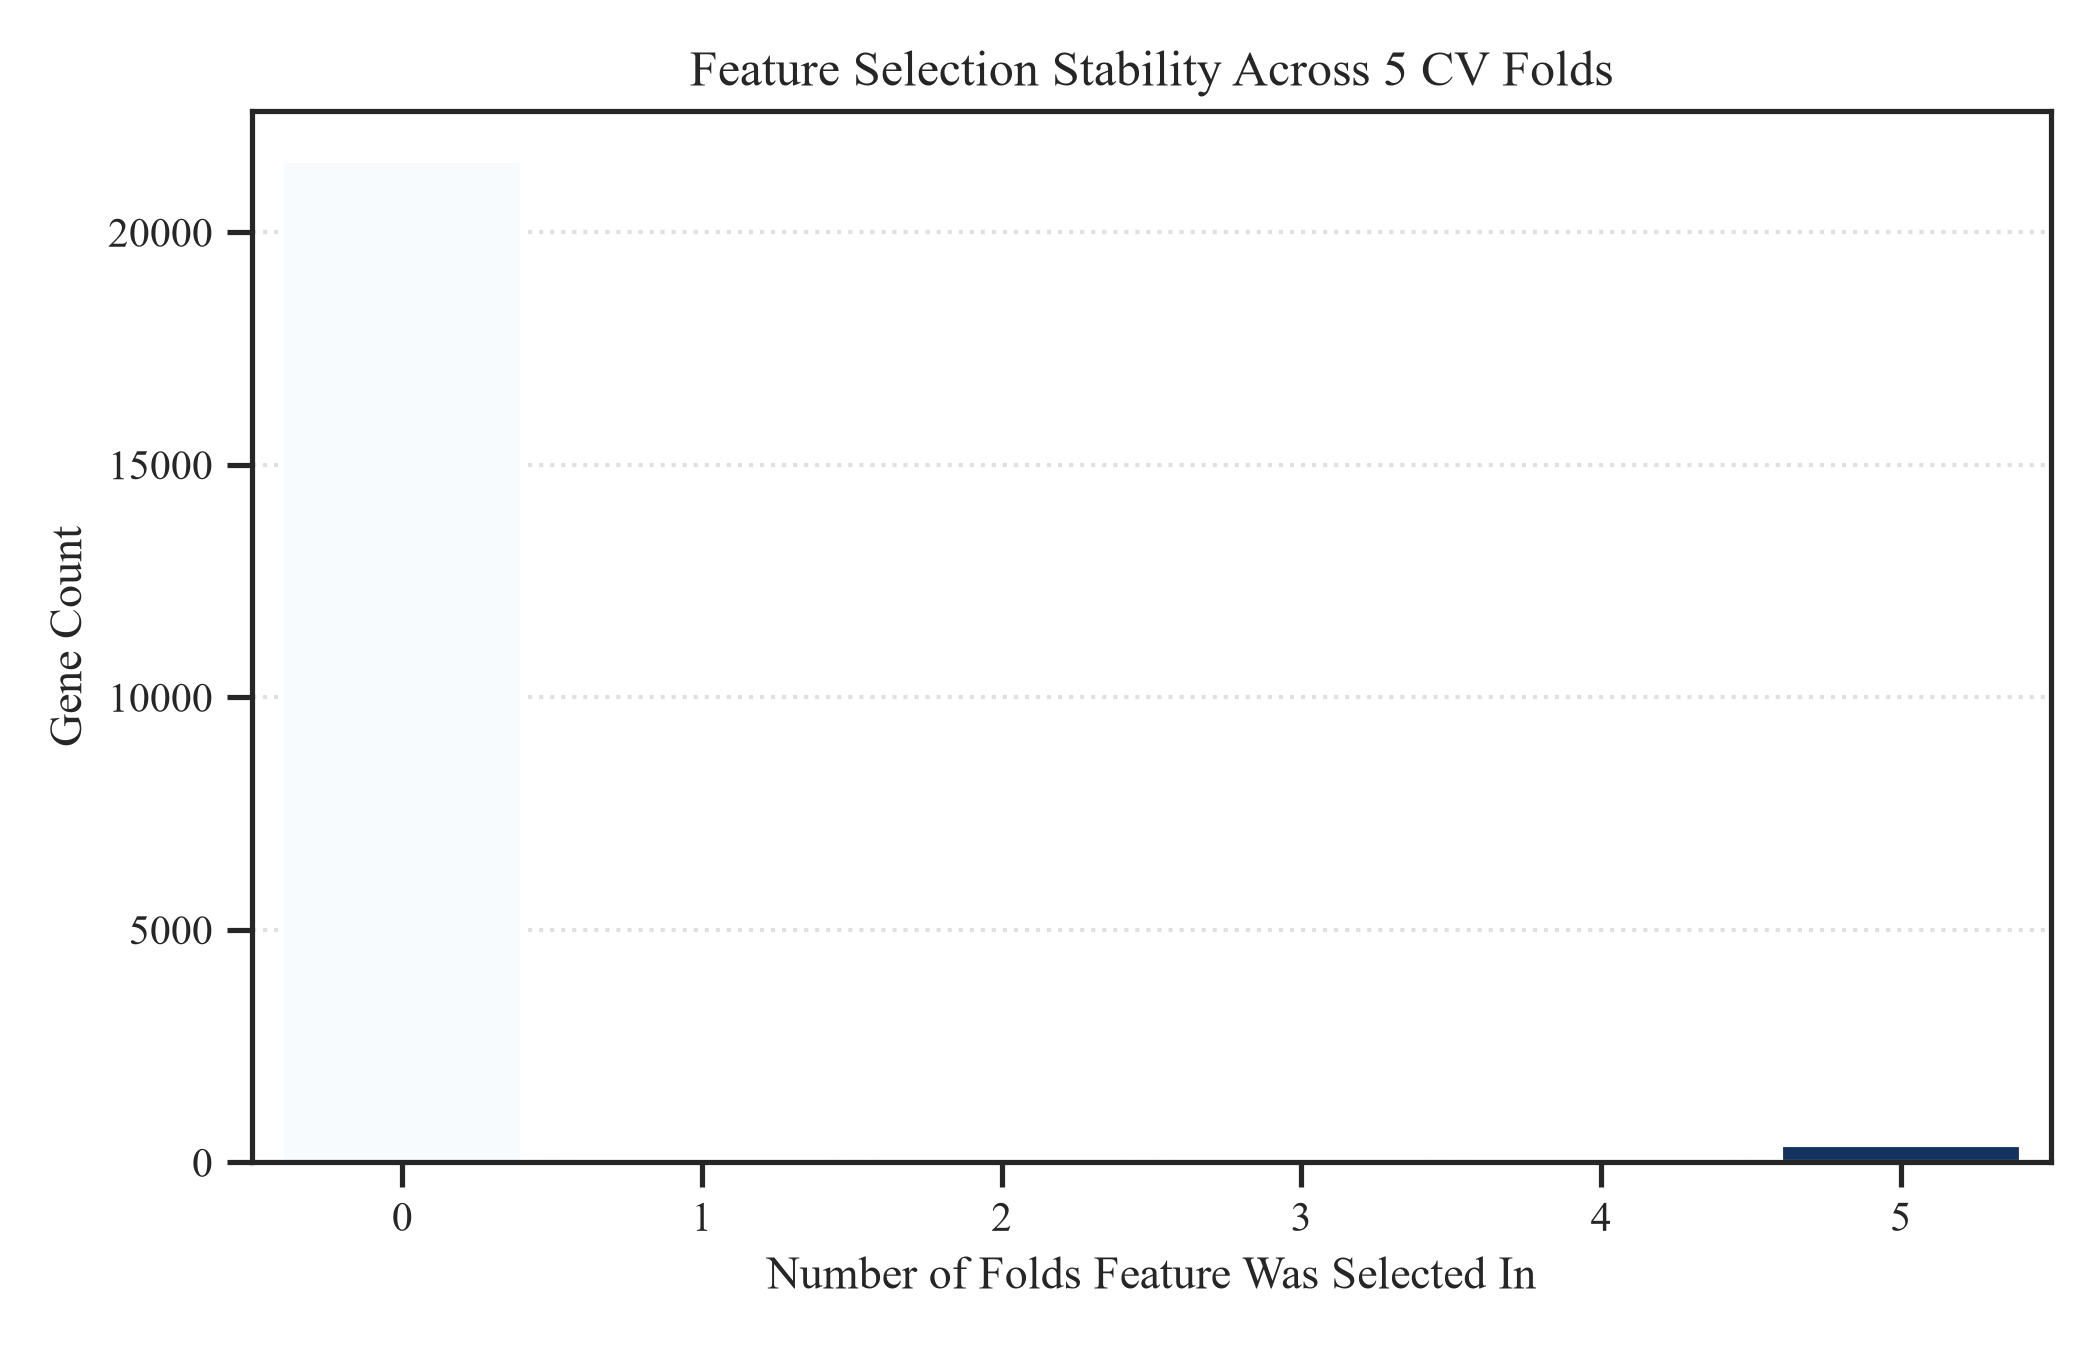
\includegraphics[width=0.78\columnwidth]{feature_selection_stability.png}
\end{center}
\end{block}

\vspace*{0.25cm}

\begin{block}{External Validation: GEO $\rightarrow$ TCGA}
\begin{center}
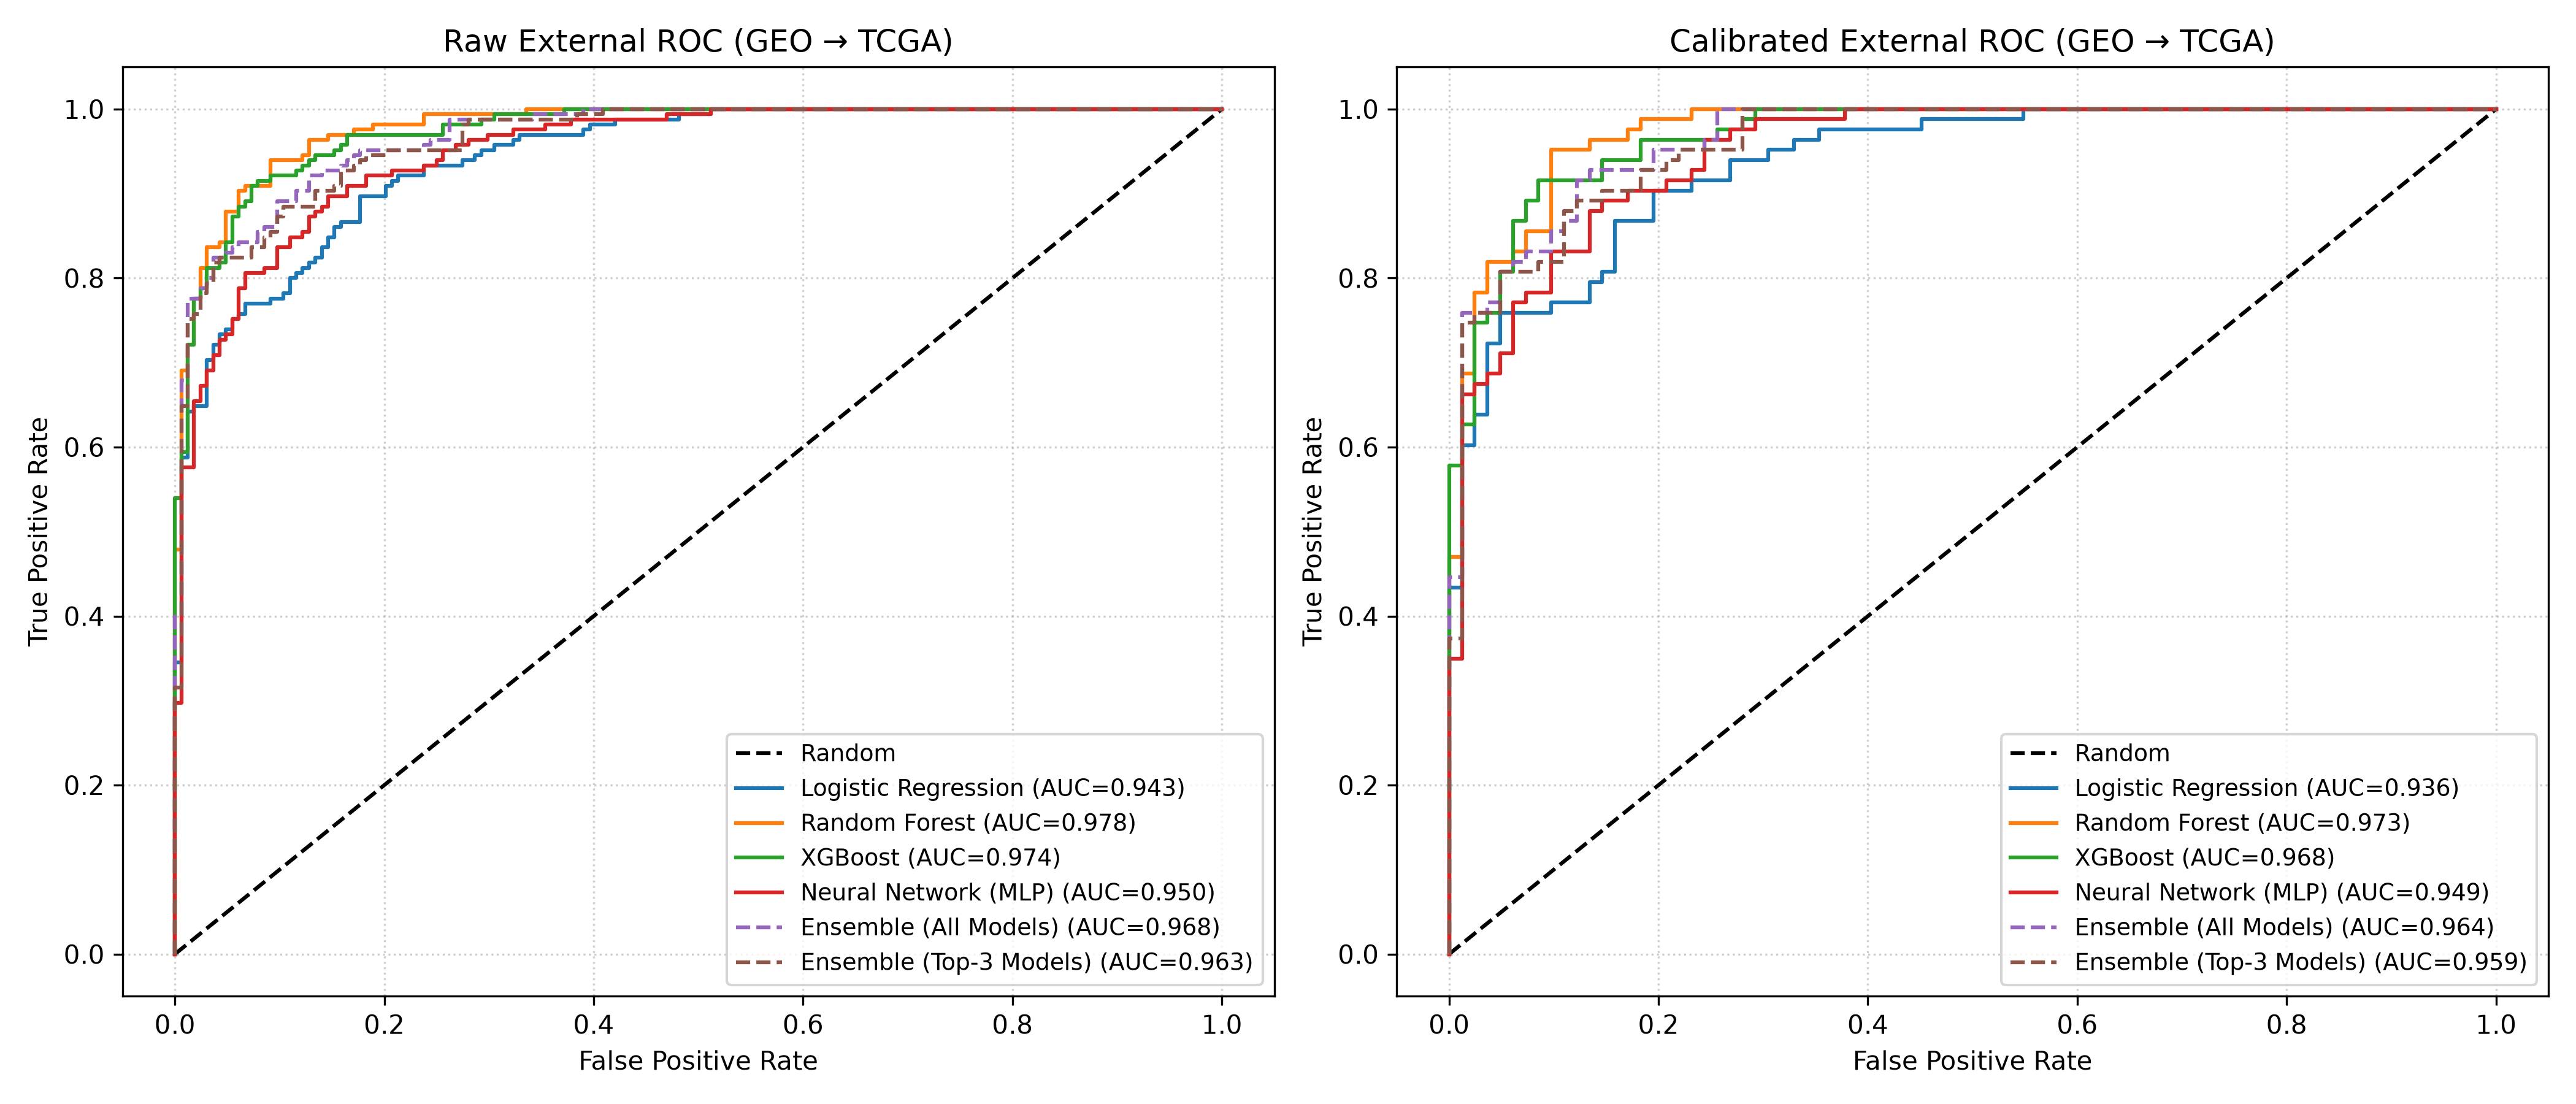
\includegraphics[width=0.71\columnwidth]{external_roc_geo_to_tcga.png}
\end{center}
\textbf{Cross-Platform AUCs (GEO Affymetrix $\rightarrow$ TCGA RNA-seq)}
\begin{center}
\small
\begin{tabular}{lcc}
\toprule
Model & Raw AUC & Calibrated AUC \\
\midrule
Logistic Regression & 0.936 & 0.937 \\
Random Forest & \textbf{0.973} & \textbf{0.973} \\
XGBoost & 0.968 & 0.968 \\
MLP & 0.949 & 0.949 \\
\bottomrule
\end{tabular}
\end{center}
\end{block}

\vspace*{0.25cm}

\begin{block}{Calibration Benchmark Results}
\textbf{Key Finding: Platt Scaling Significantly Reduces ECE}
\begin{itemize}
\item \textbf{RF Platt:} AUC=0.973, ECE=0.043 --- 95\% CIs non-overlapping with uncalibrated (ECE=0.115)
\item \textbf{LR QN+Platt:} AUC=0.972 --- best cross-platform transfer calibration
\end{itemize}
\begin{center}
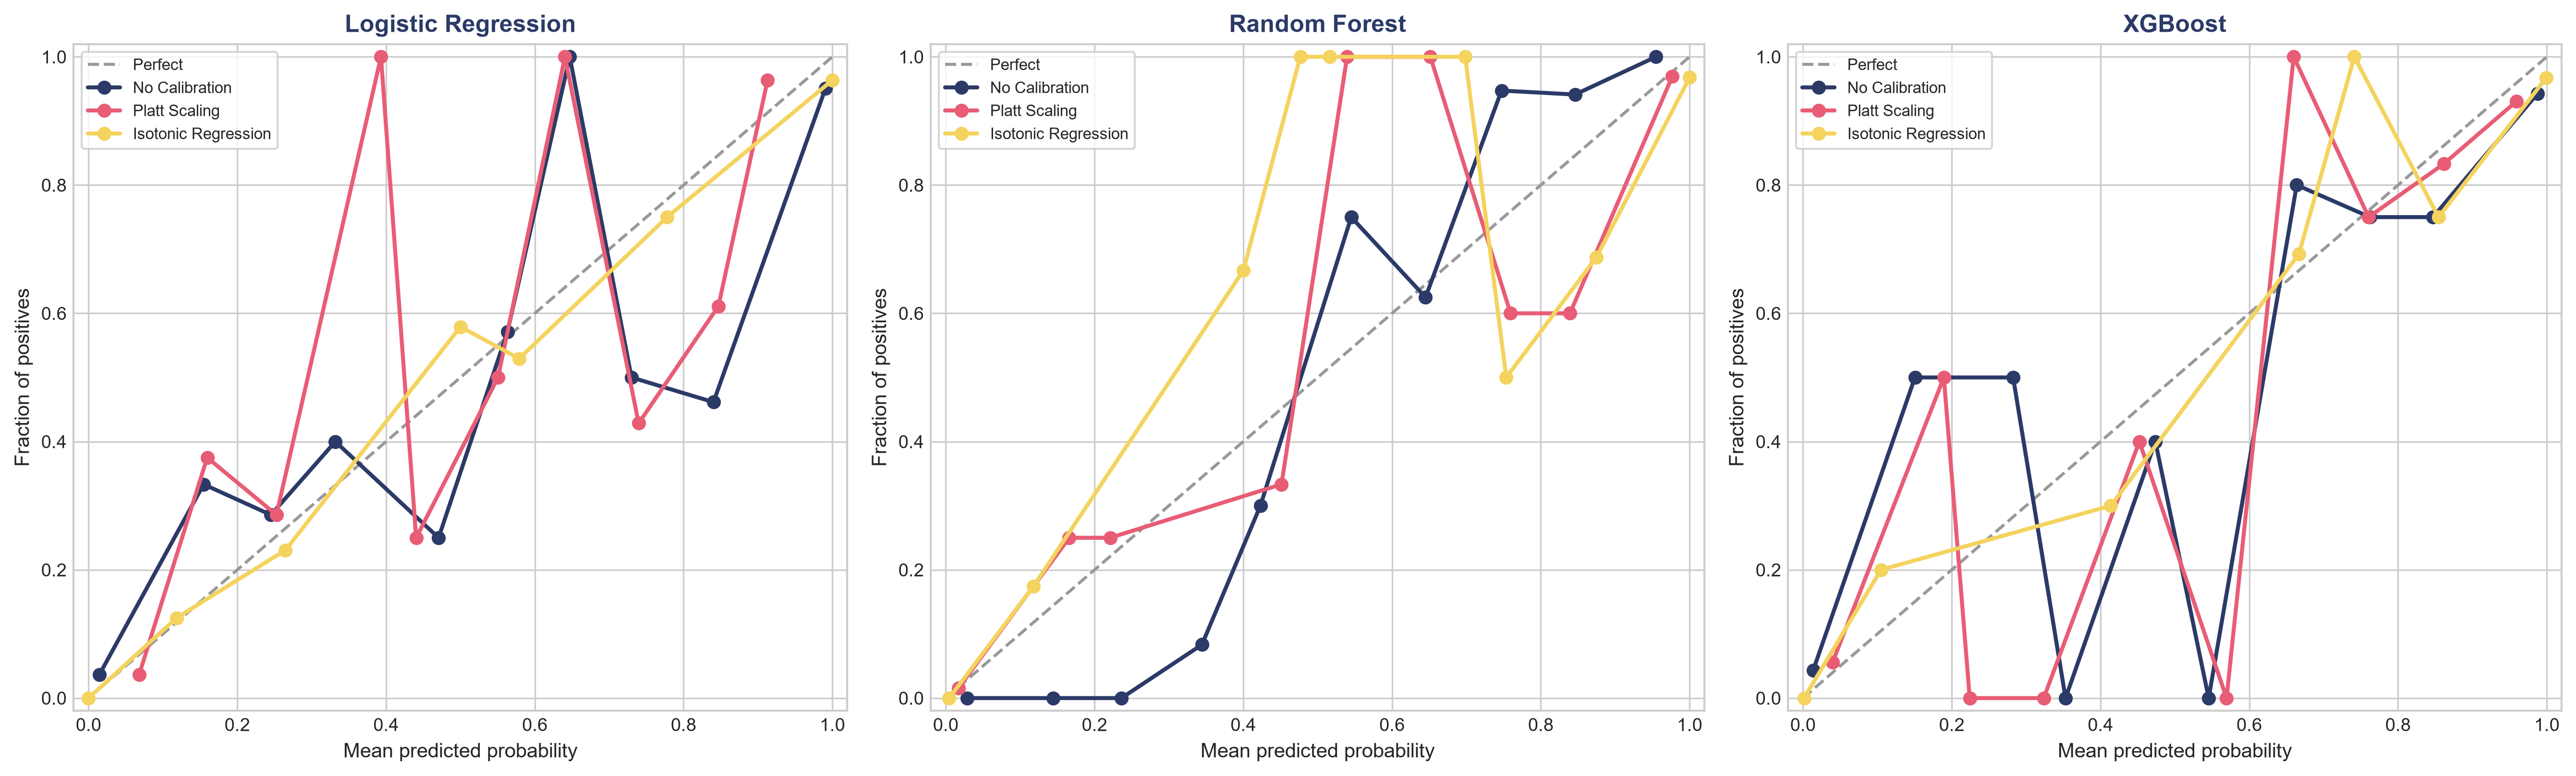
\includegraphics[width=0.70\columnwidth]{calibration_benchmark.png}
\end{center}
\textbf{Best Config per Model (sorted by ECE)}
\begin{center}
\small
\begin{tabular}{llll}
\toprule
Model & Calibration & AUC & ECE \\
\midrule
RF & Platt & 0.973 & 0.043 \\
XGBoost & Platt & 0.968 & 0.038 \\
MLP & Isotonic & 0.935 & 0.029 \\
LR & Isotonic & 0.925 & 0.028 \\
\bottomrule
\end{tabular}
\end{center}
\end{block}
\end{column}

% --------------------------- Column 3 (narrow) ---------------------------
\begin{column}{0.27\textwidth}
\begin{block}{Ablation: StabilitySelector vs SelectKBest}
\begin{center}
\small
\begin{tabular}{lll}
\toprule
Selector & Model & Holdout AUC \\
\midrule
\textbf{SS} & Logistic Regression & \textbf{0.994} \\
SKB & Logistic Regression & 0.994 \\
\textbf{SS} & Random Forest & \textbf{0.988} \\
SKB & Random Forest & 0.988 \\
\textbf{SS} & XGBoost & \textbf{0.990} \\
SKB & XGBoost & 0.991 \\
\textbf{SS} & MLP & \textbf{0.992} \\
SKB & MLP & 0.983 \\
\bottomrule
\end{tabular}
\end{center}

SS matches or beats SKB on all 4 models. \textbf{MLP: +0.009 AUC (0.983 $\rightarrow$ 0.992).}

\vspace{0.1cm}
\textbf{Minimal Panel (LASSO):} \textbf{LASSO $\rightarrow$ 83 genes, AUC 0.985} (full 500-gene pipeline: 0.983). Most stable: KIF23, DNA2, MCM3 --- replication/mitosis machinery, no label genes.

\vspace{0.1cm}
\textbf{LASSO Gene Stability}
\begin{center}
\small
\begin{tabular}{lc}
\toprule
Gene & Selection frequency \\
\midrule
KIF23 & 1.00 \\
DNA2 & 0.97 \\
MCM3 & 0.97 \\
DDIAS & 0.93 \\
SNRPB & 0.90 \\
\bottomrule
\end{tabular}
\end{center}
30 of the 83 LASSO genes were selected in $\geq 50\%$ of bootstrap resamples --- replication and mitosis machinery, none from the label signature.
\end{block}

\vspace*{0.15cm}

\begin{block}{Survival Power Analysis (Schoenfeld)}
\begin{center}
\small
\begin{tabular}{lcc}
\toprule
Cohort & Events & Log-rank $p$ \\
\midrule
GSE39582 (GEO) & 194 & 0.037 \\
TCGA-COAD & 79 & 0.034 \\
TCGA PanCancer & 100 & 0.009 \\
CPTAC-COAD & 7 & 0.356 \\
\bottomrule
\end{tabular}
\end{center}

Univariate log-rank tests were adequately powered (79--194 events). The CPTAC null (7 events) is underpowered --- do not over-interpret.
\end{block}

\vspace*{0.15cm}

\begin{block}{Survival Analysis}
\begin{center}
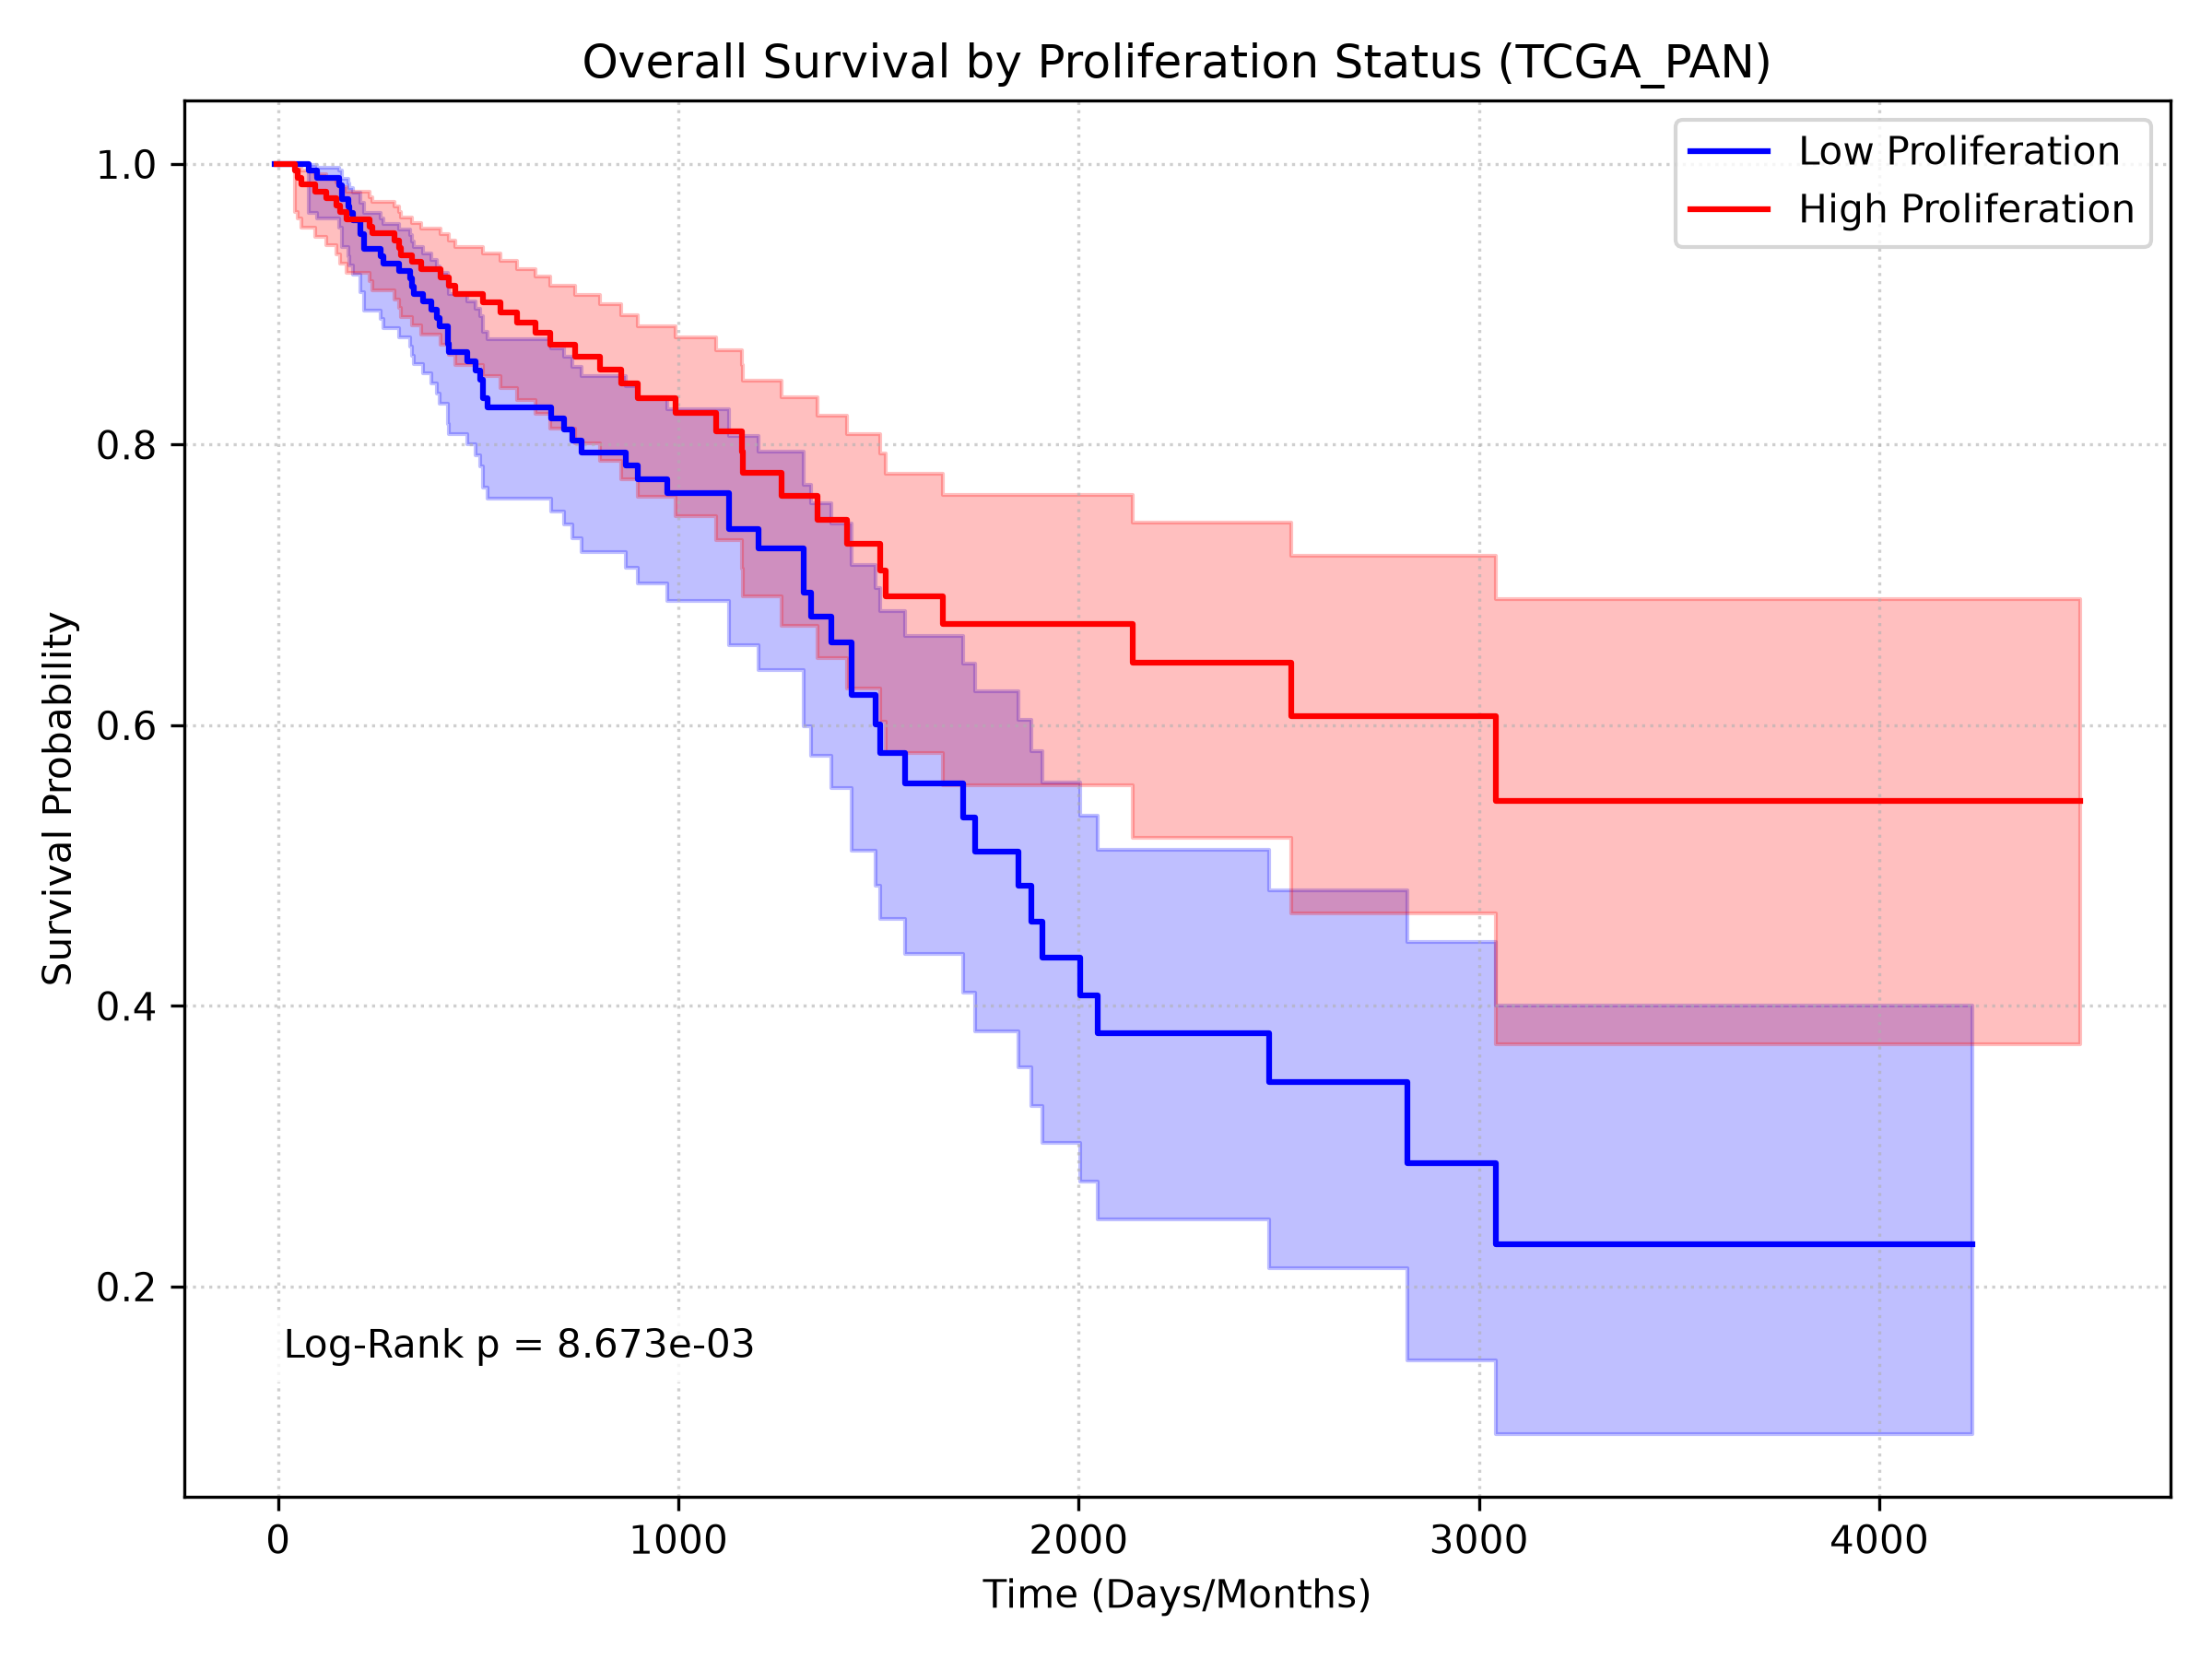
\includegraphics[width=0.42\columnwidth]{kaplan_meier_tcga_pan.png}
\end{center}
\textbf{Significant stratification (Log-Rank $p < 0.05$)} --- worse overall survival for the high-proliferation group in TCGA ($p=0.009$) and GEO ($p=0.037$). Cox PH adjusted for stage: HR $= 0.84$, $p = 0.31$ (not independent of staging). \emph{Analysis uses the 10-gene proliferation score; model predictions give identical results (AUC $> 0.97$).}
\end{block}

\vspace*{0.15cm}

\begin{block}{Limitations \& Future Work}
\begin{itemize}
\item \textbf{Cox adjusted: not independent of stage} (HR=0.84, $p=0.31$)
\item \textbf{CPTAC} --- only 7 survival events
\item \textbf{Drug sensitivity} uses tissue type as proxy; future work will stratify by predicted proliferation score within colon lines
\item \textbf{Prospective validation} needed before clinical translation
\end{itemize}
\end{block}

\vspace*{0.15cm}

\begin{block}{References (Selected)}
\footnotesize
\begin{itemize}
\item Marisa et al.\ \emph{PLoS Med} 2013 --- GSE39582
\item Smith et al.\ \emph{Gastroenterology} 2010 --- GSE17538
\item TCGA Network. \emph{Nature} 2012 --- TCGA-COAD
\item Platt. \emph{NIPS} 1999 --- Platt scaling
\item Meinshausen \& B\"uhlmann. \emph{JRSS-B} 2010 --- stability selection
\item Iorio et al.\ \emph{Cell} 2016 --- GDSC2
\item Van Calster et al.\ \emph{BMC Med} 2019 --- clinical calibration
\item Schoenfeld. \emph{Biometrics} 1983 --- survival power
\item Tibshirani. \emph{JRSS-B} 1996 --- LASSO minimal panel
\end{itemize}
\textbf{Full list: github.com/Ronisnotasianfr/ColoGrowth-ML}
\end{block}
\end{column}

\end{columns}
\end{frame}
\end{document}
